\setcounter{chapter}{1}
\chapter[]{过程通道技术}


\section{概述}

过程通道是计算机和生产过程之间设置的信息传送和转换的连接通道,如图\ref{fig_2_01}所示。


\begin{figure}[h]
  \centering
  % Requires \usepackage{graphicx}
  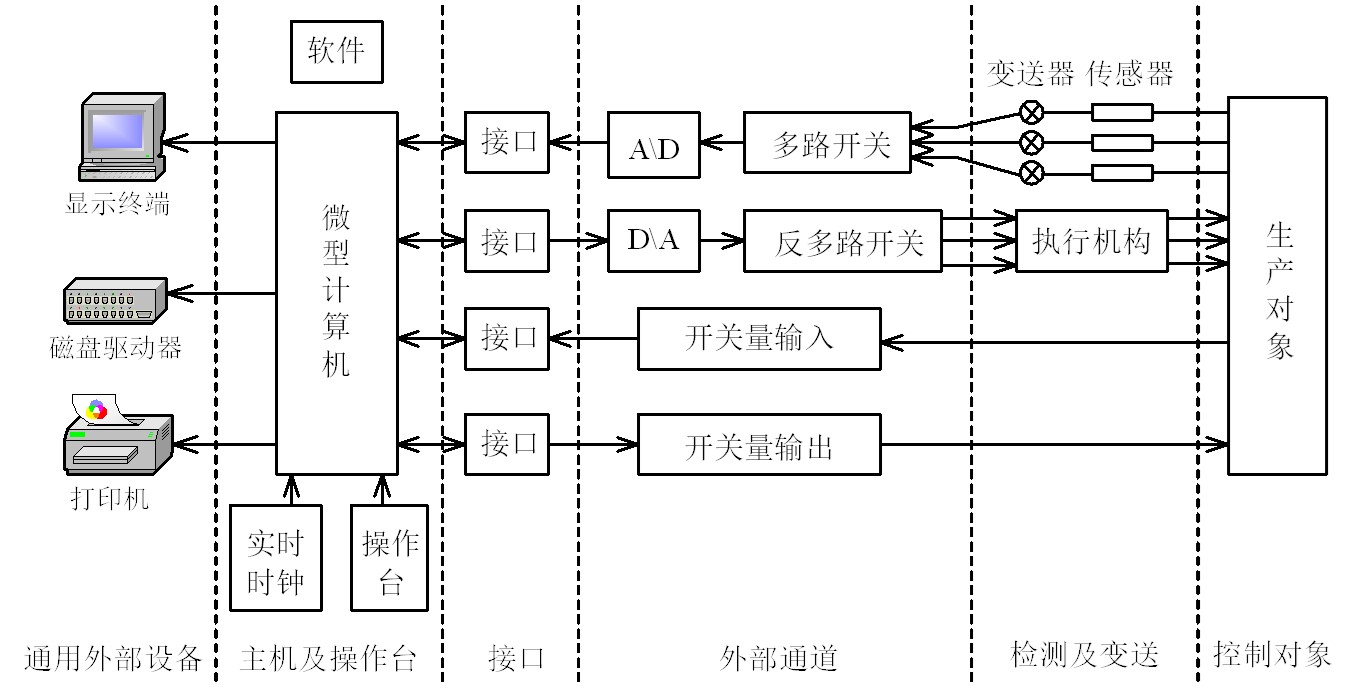
\includegraphics[width=0.8\textwidth]{fig_2_01}\\
  \caption{过程通道}\label{fig_2_01}
\end{figure}



过程通道包括:
\begin{table}[h]
  \centering
  \begin{tabular}{|c|c|}
  \hline
  % after \\: \hline or \cline{col1-col2} \cline{col3-col4} ...
  检测通道/输入通道 & 控制通道/输出通道 \\  \hline

     数字量输入通道& 数字量输出通道\\

     脉冲量输入通道& 脉冲量输出通道\\

     模拟量输入通道& 模拟量输出通道\\  \hline
\end{tabular}

  \caption{过程通道}\label{tab:2.1}
\end{table}

其中,脉冲量有时也作为数字量处理。





\section{通道接口技术}




\subsection{通道地址译码技术}

\begin{remark}
  为什么需要编址和译码?

  以通道接口的观点看,CPU与输入/输出通道的关系是一对多,而非一对一。如果要对其中某一个通道进行输入/输出操作,就需要给每个通道接口设定一个地址,即为编址。当CPU需要操作一个通道接口时,就可利用CPU总线输出一个该地址,配合数字组合逻辑电路,产生一个使能信号(Enable)或称选通信号(Select)使该地址对应的通道接口可与CPU进行数据的交换。
\end{remark}

\subsubsection{编址方式}

\begin{itemize}
  \item 存储器统一编址方式(WR、RD)

存储器指令丰富,使用灵活,程序设计方便;占用了存储空间地址,指令执行时间较长,难以区分I/O操作。

  \item I/O接口编址方式(MREQ、IORQ配合WR和RD或IOW、IOR)

I/O指令简单,执行时间短,硬件设计简单,程序设计清晰;输入输出数据必须经过累加器A。

\end{itemize}



\subsubsection{地址译码}

\begin{enumerate}
  \item 译码器译码
  \begin{itemize}
    \item 适合连续多个地址的译码电路设计
    \item 常用的译码器芯片:3-8译码器74LS138;74LS154,是4-16译码器


    \item \textbf{3-8译码器举例}
  \end{itemize}



  \item 通用阵列逻辑(GAL:Generic Array Logic)器件译码:由译码器构成的译码电路虽能很好地完成译码功能。但都需要非止一个器件来构成译码电路。在实际应用中需要较大的安装空间和较多种类的产品备件.这将影响最终产品的成本、可靠性及可维护性。
\begin{itemize}
  \item 具有可编程的与门及或门阵列;
  \item 可定义每个输出引脚的结构和功能;
  \item GAL器件可在线电擦写、编程,数据保持时间在10年以上;
  \item GAL器件有较高的响应速度,与TTL兼容;
  \item GAL器件具有可编程的保密位,防止非法读取和复制。
  \item 常用GAL器件:GAL16v8、GAL20v8

\end{itemize}

\end{enumerate}


\textbf{例:3-8译码器举例}: 74LS138译码器的管脚图及真值表见下图:

\begin{figure}[h]
  \centering
  % Requires \usepackage{graphicx}
  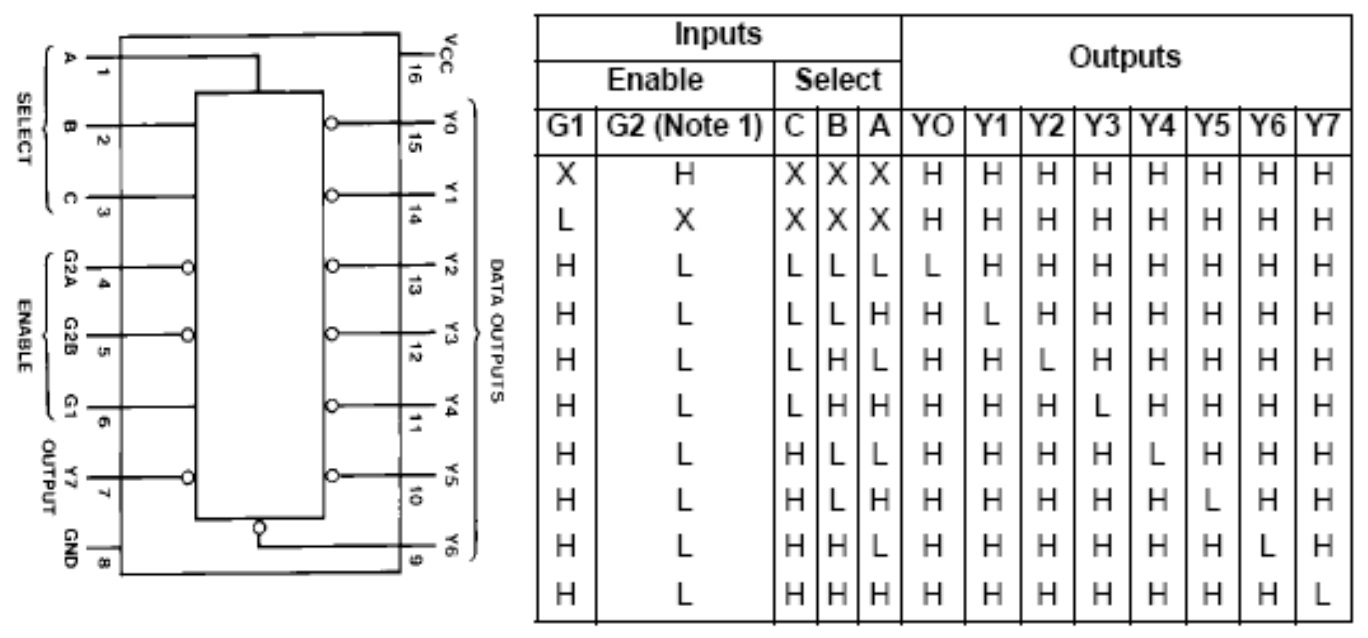
\includegraphics[width=0.5\textwidth]{74ls138}\\
  \caption{74LS138译码器}\label{fig:138_1}
\end{figure}

掌握一种数字逻辑电路芯片的关键是读懂其真值表。首先,了解一些术语的含义,参见下表。其次,解读其使用方法。例如,要想使74LS138工作,必然要求满足G1=H、G2=L,否则不管C/B/A为何值,输出Y0-Y7都一直为H。当满足G1=H、G2=L 后,输出Y0-Y7会随着C/B/A 的变化。最后,根据输入/输出的关系,设定Y0-Y7的地址,应是水到渠成。

\begin{table}[h]
  \centering
\begin{tabular}{|l|l|}
  \hline
  % after \\: \hline or \cline{col1-col2} \cline{col3-col4} ...
  H: 高电平 & L: 低电平 \\
  X: Don't care/无作用 & Z: 高阻态 \\
  Enable: 使能 & Select:选择/选通 \\
  \hline
\end{tabular}
  \caption{真值表常用术语}\label{tab:2.2}
\end{table}


以下图为例,考虑:
\begin{enumerate}
  \item 要求Y0-Y7能够在地址总线输出2E0H-2E7H时分别实现使能,应当如何连接?
  \item 或者,反过来,当采用如图的连接时,Y0-Y7分别对应什么地址?
\end{enumerate}


\begin{figure}[h]
  \centering
  % Requires \usepackage{graphicx}
  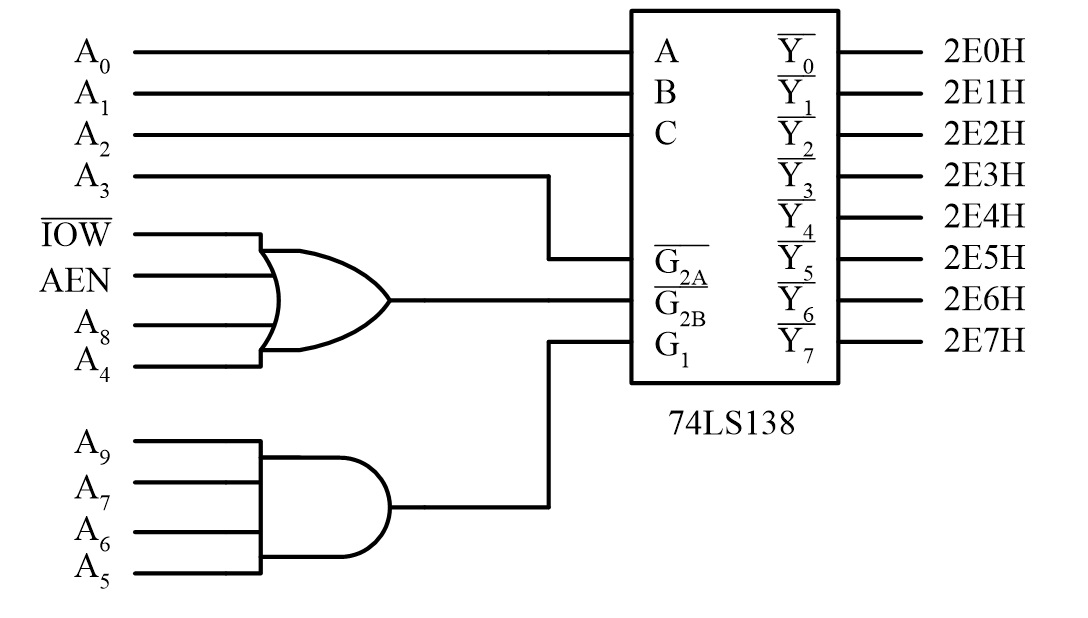
\includegraphics[width=0.5\textwidth]{74ls138_2}\\
  \caption{74LS138译码器使用举例}\label{fig:138_2}
\end{figure}




需要的知识:
\begin{itemize}
  \item A0-A9共10位,为地址总线
  \item AEN为地址总线使能,使能时为低电平
  \item $\overline{IOW}$为写IO功能,使能时为低电平。
  \item 74LS138的管脚同理
  \item 与门:所有输入均为1,输出才为1;或者说,要满足输出为1,所有输入必为1
  \item 或门:……
\end{itemize}

到此为止,以大家的智商,应该可以解决以上两个问题。进一步,应该形成一个解决问题的方法。

\begin{enumerate}
  \item 将地址写为二进制形式,例如:$2E0H-2E7H=01,1110,0XXXB$;
  \item 将C/B/A对应A2/A1/A0(注意:仅连续译码时才是这种连接);
  \item 将应为0的信号(包括A3-A9,${AEN}$,$\overline{IOW}$)与$\overline{G2A}$或$\overline{G2B}$或对应的四输入或门相连。
  \item 将应为1的信号与G1或对应的四输入与门相连。
\end{enumerate}

\begin{remark}
  74LS138芯片是为实现连续地址译码设计的芯片,但也可以实现非连续地址的译码。如何实现,可参见数电课程中的相关知识,通过增加相应的数字电路实现。
\end{remark}



\subsection{总线接口常用芯片}


在应用系统中,几乎所有系统扩展的外围芯片都是通过总线与CPU连接的,但是:


\begin{itemize}
  \item  总线的数目是有限的;

  \item 外围芯片工作时有一个输入电流,不工作时也有漏电流存在,因此总线只能带动一定数量的电路;

  \item 对于多电压系统,不同电平标准芯片的连接也需要电平的匹配;

\end{itemize}


\begin{remark}

一.TTL

      TTL集成电路的主要型式为晶体管-晶体管逻辑门(transistor-transistor logic gate),TTL大部分都采用5V电源。

      1.输出高电平Uoh和输出低电平Uol

      $U_{oh}\ge 2.4~V$, $U_{ol}\le 0.4~V$

      2.输入高电平和输入低电平

      $U_{ih}\ge 2.0~V$,$U_{il}\le 0.8~V$

二.CMOS

      CMOS电路是电压控制器件,输入电阻极大,对于干扰信号十分敏感,因此不用的输入端不应开路,接到地或者电源上。CMOS 电路的优点是噪声容限较宽,静态功耗很小。

1.输出高电平Uoh和输出低电平Uol

$Uoh\approx VCC$,$Uol\approx GND$

2.输入高电平Uoh和输入低电平Uol

$U_{ih}\ge 0.7~VCC$,$U_{il}\le 0.2~VCC$

(VCC为电源电压,GND为地)

\end{remark}

\subsubsection{锁存器}

74LS574、74LS573\newline

\begin{figure}[h]
  \centering
  % Requires \usepackage{graphicx}
  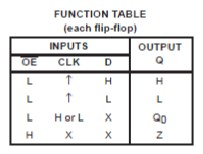
\includegraphics[height=0.2\textwidth]{fig_2_574}(a)
  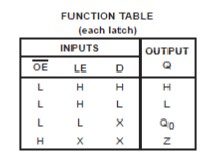
\includegraphics[height=0.19\textwidth]{fig_2_573}(b)\\
  \caption{74LS574(a)/573(b)锁存器的真值表}\label{fig:fig_2_574}
\end{figure}



\begin{remark}
锁存器可将数据锁定在其输出端,使数据稳定下来保持一段时间不变化,直到CPU用新的数据将其替换,用于实现数据从CPU到外设的传送。
\end{remark}

\subsubsection{缓冲器}

74LS244、74LS245\newline


\begin{figure}[h]
  \centering
  % Requires \usepackage{graphicx}
  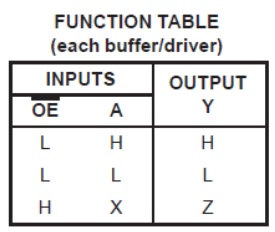
\includegraphics[height=0.2\textwidth]{fig_2_244}(a)
  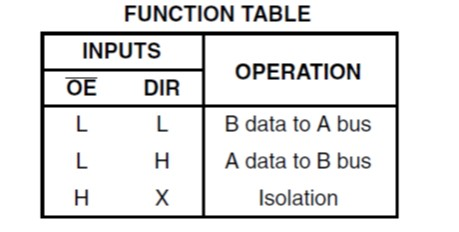
\includegraphics[height=0.17\textwidth]{fig_2_245}(b)\\
  \caption{74LS244(a)/245(b)缓冲器的真值表}\label{fig:fig_2_244}
\end{figure}



\begin{remark}
缓冲器可以使高速工作的CPU与慢速工作的外设 协调工作,实现数据从外设到CPU的传送。由于缓冲器的输出接在数据总线上,故必须具有三态输出功能。为什么?


三态输出门具有‘1’,‘0’,‘Z’三种输出状态。其中,高阻态‘Z’用于器件间信号隔离,当需要隔离的时候就置输出为‘Z’ 态,那么其他器件的信号就不会对本器件内数据构成影响,例如一条数据总线上连接有两片缓冲器(甲和乙),甲在输出给CPU时,乙就要置输出为‘Z’态,否则甲/乙的输出电平会在数据总线上产生冲突。

\end{remark}



\section{数字量输入通道}

\subsection{数字量输入通道的结构}



什么芯片可实现这里的输入缓冲?
\begin{figure}[h]
  \centering
  % Requires \usepackage{graphicx}
  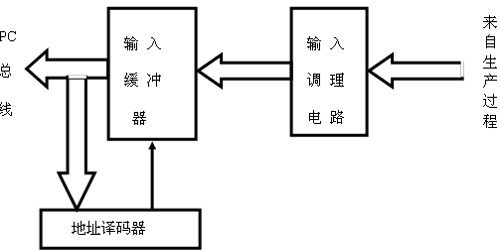
\includegraphics[width=0.5\textwidth]{fig_2_02}\\
  \caption{数字量输入通道的结构}\label{fig_2_02}
\end{figure}


\subsection{数字量输入调理电路}
\textbf{信号调理}:将现场输入的信号经转换、保护、滤波、隔离等措施转换成计算机能够接收的逻辑信号。可能引入瞬时的高压、过电压、接触抖动等现象。开关量(数字量)的种类:
\begin{itemize}
  \item 按类型分有电平式和触点式两种
  \begin{itemize}
    \item 电平式为高电平或低电平
    \item 触点式为触点闭合或触点断开
  \end{itemize}
  \item 按电源分有有源和无源两种
  \begin{itemize}
    \item 有源即直接提供高、低电平

    \item 无源即提供物理触点,或感应器件

  \end{itemize}

\end{itemize}


\subsubsection{对抖动的调理}

两种常用的方法,如图\ref{fig_2_03}所示。
\begin{enumerate}
  \item 利用RC滤波电路
  \item 利用R-S双稳态触发电路
\end{enumerate}



\begin{figure}[h]
  \centering
  % Requires \usepackage{graphicx}
  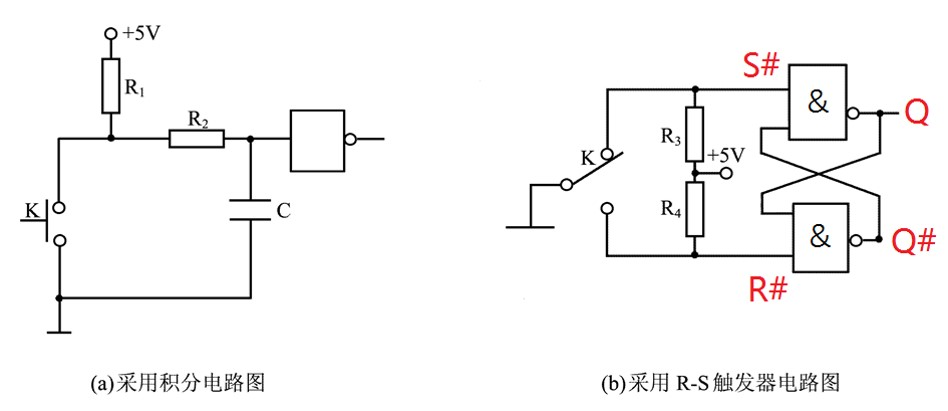
\includegraphics[width=0.6\textwidth]{fig_2_03}\\
  \caption{消抖电路}\label{fig_2_03}
\end{figure}

\begin{remark}
  R-S双稳态触发电路如何消抖?
\begin{itemize}
  \item 开关K可以使$S\#$和$R\#$处于何种状态;
  \item R-S双稳态触发电路的性质,参见图\ref{fig_2_rs}(a);
  \item 考虑正常情况和非正常(按键K出现抖动)情况下,电路的输出如何响应。
\end{itemize}
\end{remark}

\begin{figure}[h]
  \centering
  % Requires \usepackage{graphicx}
  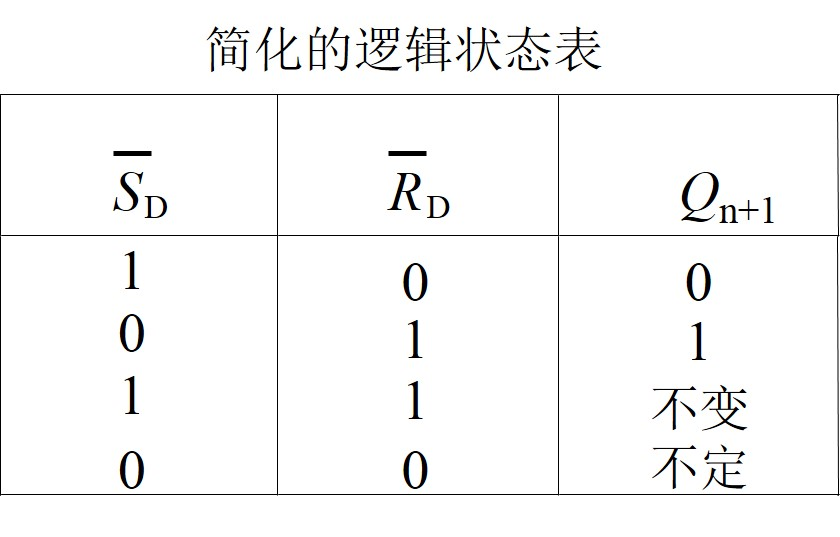
\includegraphics[width=0.35\textwidth]{fig_2_rsa}(a)
  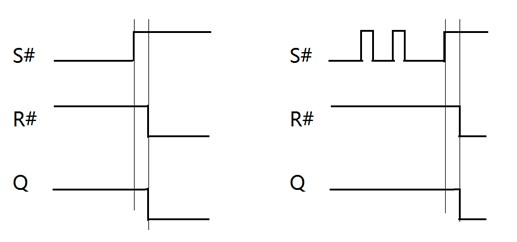
\includegraphics[width=0.45\textwidth]{fig_2_rs}(b)\\
  \caption{双稳态触发电路消抖的原理}\label{fig_2_rs}
\end{figure}

\subsubsection{保护}

数字量输入通道常用的保护电路,如图\ref{fig_2_04}所示。理解各元件的保护功能,可以从各元件的伏安特性曲线入手。常见的电阻是典型的线性元件,满足$U=IR$;各种二极管、三极管和压敏电阻则是非线性元件,合理的使用可起到保护主要电路的作用。


\begin{figure}[h]
  \centering
  % Requires \usepackage{graphicx}
  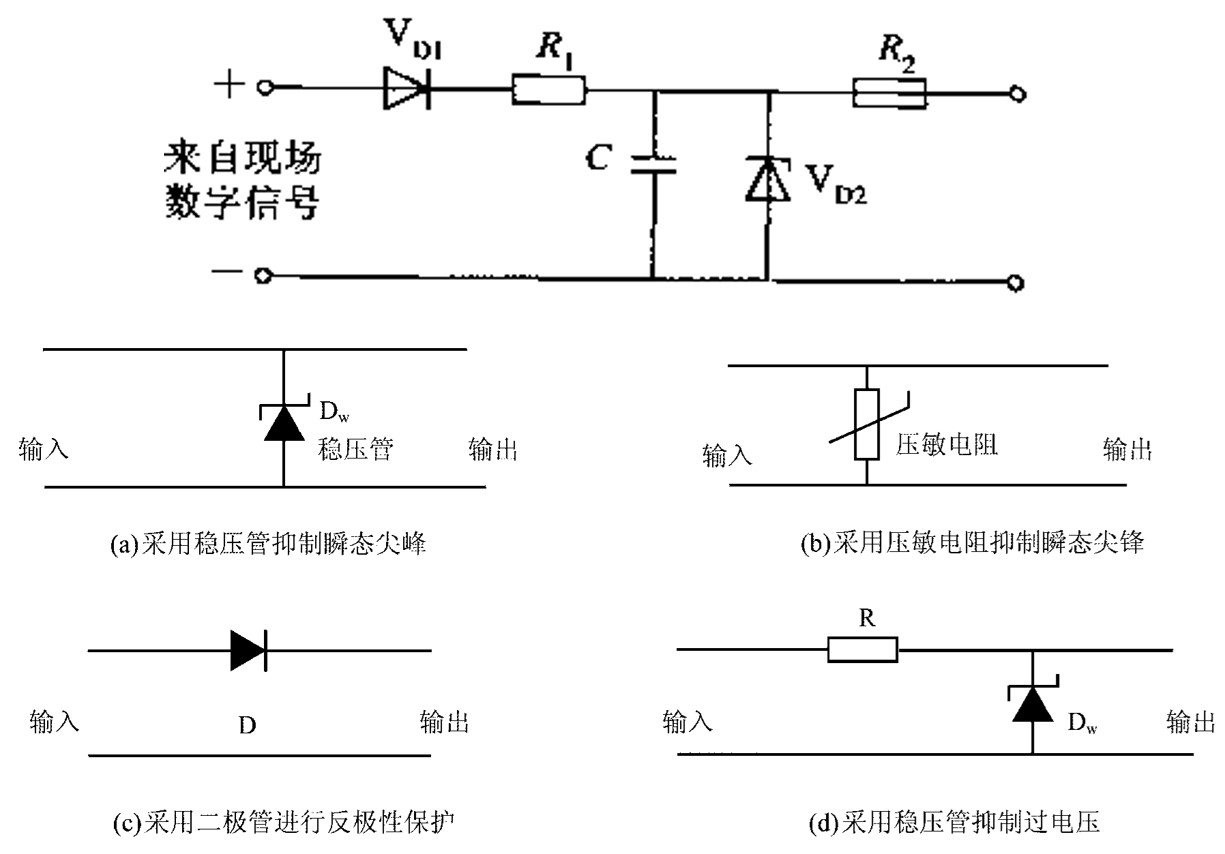
\includegraphics[width=0.6\textwidth]{fig_2_04}
  \caption{保护电路}\label{fig_2_04}
\end{figure}



以稳压二极管为例,其伏安特性如图\ref{fig_2_04a}所示。稳压二极管的特点就是被反向击穿后,其两端的电压基本保持不变。这样,当把稳压管接入电路以后,若由于电源电压发生波动,或其它原因造成电路中各点电压变动时,负载两端的电压将基本保持不变。

\begin{figure}[h]
  \centering
  % Requires \usepackage{graphicx}
  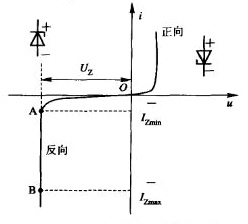
\includegraphics[width=0.3\textwidth]{fig_2_04a}
  \caption{稳压管的伏安特性}\label{fig_2_04a}
\end{figure}


\subsubsection{隔离}

在工业现场获取的开关量或数字量的信号电平往往高于计算机系统的逻辑电平,即使输入数字量电压本身不高,也可能从现场引入意外的高压信号,因此必须采取电隔离措施,以保障系统安全。


光电耦合器,简称光耦,是一种常用且非常有效的电隔离手段,由于它价格低廉,可靠性好,被广泛地应用于现场输入设备与计算机系统之间的隔离保护。光电耦合器是把发光器件和光敏器件组装在一起,通过光实现耦合构成‘电-光’和‘光-电’转换的器件,如图\ref{fig_2_05a}(a)所示为其原理图。


\begin{figure}[h]
  \centering
  % Requires \usepackage{graphicx}
  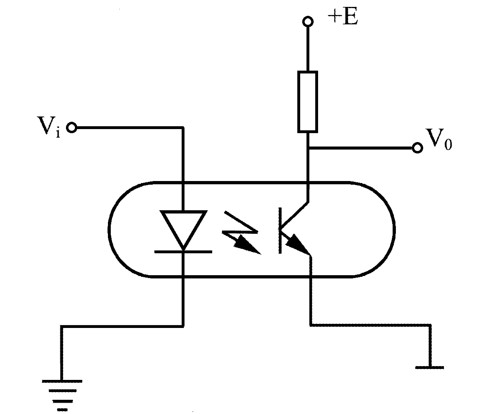
\includegraphics[width=0.2\textwidth]{fig_2_05a}(a)
  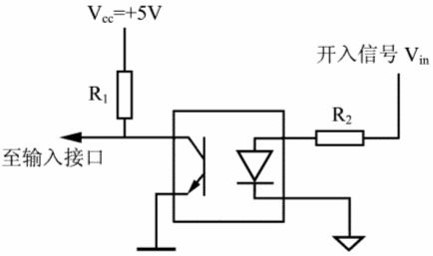
\includegraphics[width=0.3\textwidth]{fig_2_05b}(a)
    \caption{光电耦合器}\label{fig_2_05a}
\end{figure}


当电信号送入光耦输入端时,发光二极管发光,光敏器件受到光照后产生电流,ce导通;反之,ce不导通。对于数字量,输入为低电平‘0’时,光敏三极管截止,输出为高电平;反之,输出为低电平。




\begin{description}
  \item[常开] —NO(normal open)通常情况下是断开状态,即线圈未得电的情况下断开的。在常态(不通电)的情况下处于断开状态的触点叫常开触点。

  \item[常闭] —NC(normal close)通常情况下是关合状态,即线圈未得电的情况下闭合的。在常态(不通电、无电流流过)的情况下处于闭合状态的触点叫常闭触点。


\end{description}




\section{数字量输出通道}

\subsection{数字量输出通道的结构}

\begin{figure}[h]
  \centering
  % Requires \usepackage{graphicx}
  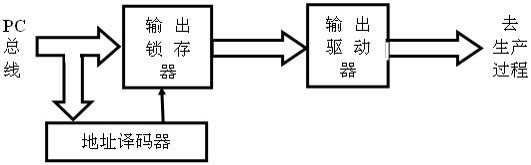
\includegraphics[width=0.5\textwidth]{fig_2_05}
  \caption{数字量输出通道的结构}\label{fig_2_05}
\end{figure}


\subsection{数字量输出调理电路}

数字量输出的信号调理主要是进行功率放大,使控制信号具有足够的功率去驱动执行机构或其它负载。

\begin{enumerate}
  \item 小功率直流驱动电路 (几十毫安级 )
\begin{figure}[h]
  \centering
  % Requires \usepackage{graphicx}
  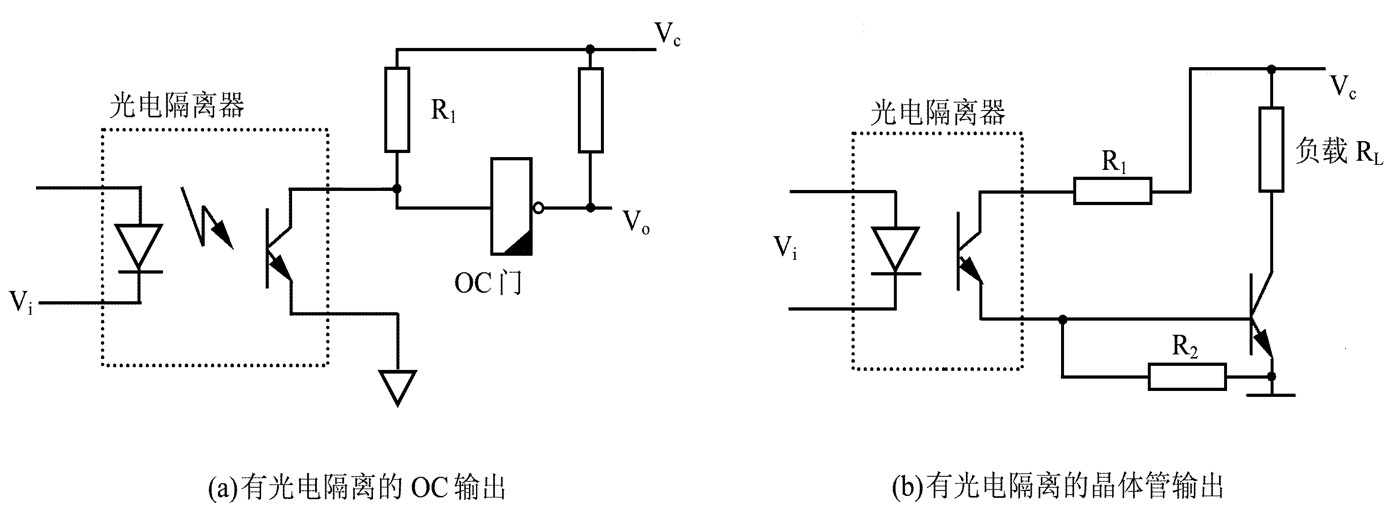
\includegraphics[width=0.6\textwidth]{fig_2_05c}
  \caption{十毫安级直流驱动电路}\label{fig_2_05c}
\end{figure}


\begin{remark}
什么是OC门?

OC门,又称集电极开路门,Open Collector,
还有OD门(Open Drain,漏极开路门,对场效应管而言)。实际使用中,有时需要两个或两个以上与非门的输出端连接在同一条导线上,将这些与非门上的数据(状态电平)用同一条导线输送出去。因此,需要一种新的与非门电路--OC门来实现“线与逻辑”。

\end{remark}

\begin{remark}
NPN与PNP三极管?


\end{remark}


  \item 继电器输出技术

      继电器经常用于计算机控制系统中的开关量输出功率放大,即利用继电器作为计算机输出的第一级执行机构,通过继电器的触点控制大功率接触器的通断,从而完成从直流低压到交流高压,从小功率到大功率的转换。

\begin{figure}[h]
  \centering
  % Requires \usepackage{graphicx}
  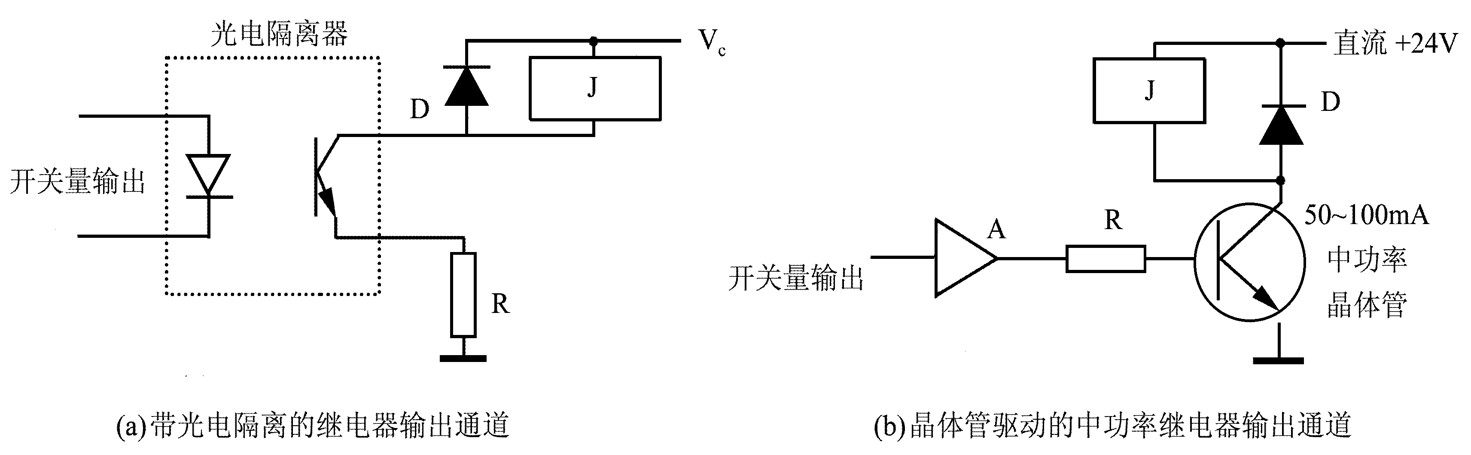
\includegraphics[width=0.6\textwidth]{fig_2_05d}
  \caption{继电器驱动}\label{fig_2_05d}
\end{figure}

\begin{remark}
二极管D的作用?续流,防止晶体管断开后线圈中的电流冲击晶体管而导致损坏。
\end{remark}

  \item 大功率交流驱动电路

      对于交流供电的负载,其开关量的输出控制可用固态继电器(Solid State Relay,SSR)来实现。


\begin{figure}[h]
  \centering
  % Requires \usepackage{graphicx}
  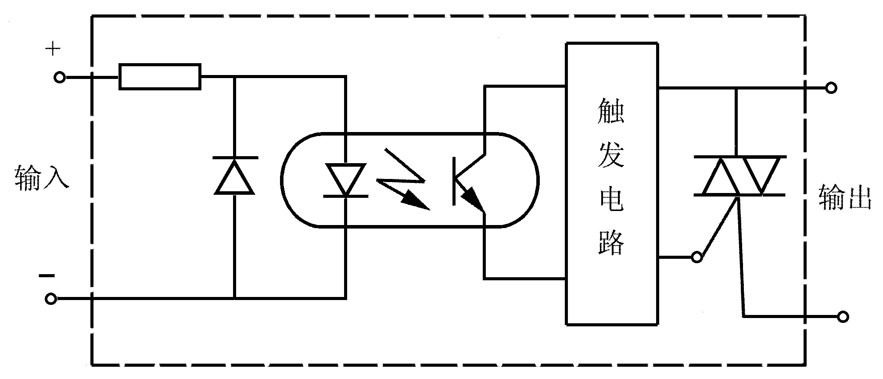
\includegraphics[height=0.1\textheight]{fig_2_05e}
  \caption{固态继电器内部结构示意图}\label{fig_2_05e}
\end{figure}


\begin{figure}[h]
  \centering
  % Requires \usepackage{graphicx}
  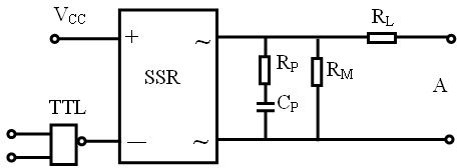
\includegraphics[height=0.1\textheight]{fig_2_05f}
  \caption{TTL驱动固态继电器}\label{fig_2_05f}
\end{figure}


\begin{figure}[h]
  \centering
  % Requires \usepackage{graphicx}
  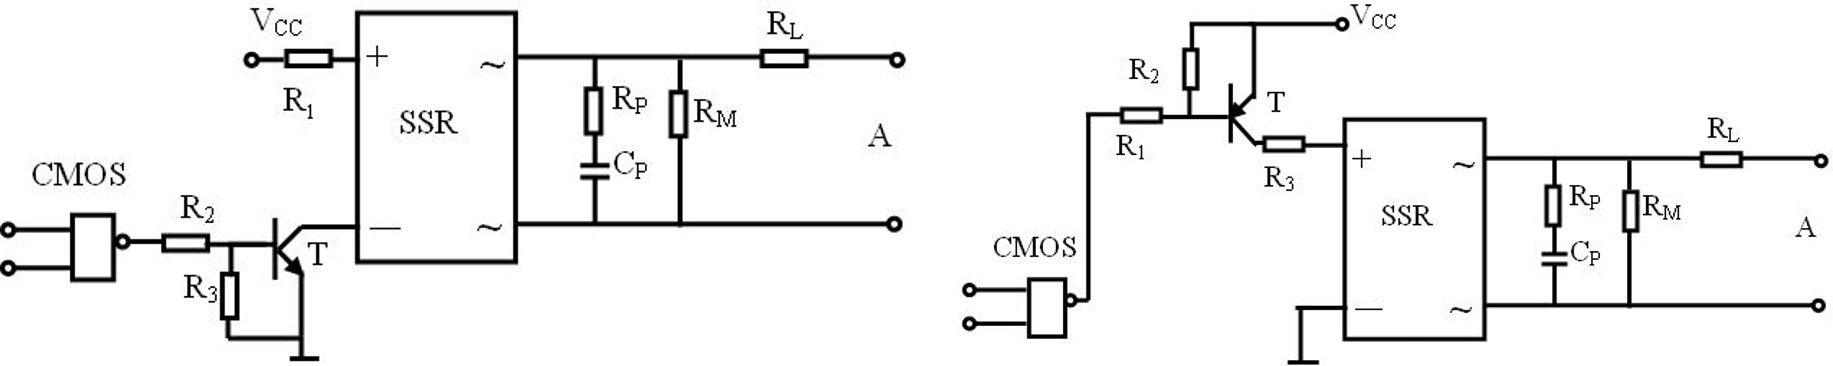
\includegraphics[height=0.1\textheight]{fig_2_05h}
  \caption{CMOS驱动固态继电器}\label{fig_2_05h}
\end{figure}

\begin{itemize}

  \item 分类:直流型(DC-SSR)节点通直流电;交流型(AC-SSR)节点通交流电。

  \item 特点:输入功率小、可靠性高、低噪声、能承受的浪涌电流大、对电源电压适应能力强(交流型对负载30V—220V)、抗扰能力强。


  \item 注意:
  \begin{itemize}
    \item 存在通态压降($<2V$);

    \item 电流负载能力随温度升高而下降,选用时留余量;

    \item SSR过载能力差,当感性负载时需加压敏电阻保护,电压选1.6~1.9 倍电源电压;
\item 输出负载短路会造成SSR损坏。

  \end{itemize}
\end{itemize}



\end{enumerate}


\begin{remark}
PNP与NPN型传感器是利用三极管的饱和和截止,输出两种状态,属于开关型传感器;其输出信号是截然相反的,即高电平和低电平。PNP与NPN型传感器一般有三条引出线,即电源线VCC、0V线,out信号输出线。在有信号触发时,NPN输出是低电平0,PNP输出的是高电平1。PNP与NPN型传感器(开关型)分为六类:
\begin{enumerate}
  \item
NPN-NO(常开型):在没有信号触发时,输出线是悬空的,就是0V线和out线断开。有信号触发时,发出与0V相同的电压,也就是out线和0V线连接,输出输出低电平0V。
  \item
NPN-NC(常闭型):在没有信号触发时,发出与0V线相同的电压,也就是out线和0V线连接,输出低电平0V。当有信号触发后,输出线是悬空的,就是0V线和out线断开。
  \item
NPN-NC+NO(常开、常闭共有型):多出一个输出线OUT,根据需要取舍。
  \item
PNP-NO(常开型):在没有信号触发时,输出线是悬空的,就是VCC电源线和out线断开。有信号触发时,发出与VCC电源线相同的电压,也就是out线和电源线VCC连接,输出高电平VCC。
  \item
PNP-NC(常闭型):在没有信号触发时,发出与VCC电源线相同的电压,也就是out线和电源线VCC连接,输出高电平VCC。当有信号触发后,输出线是悬空的,就是VCC电源线和out线断开。
  \item
PNP-NC+NO(常开、常闭共有型)其实就是多出一个输出线OUT,根据需要取舍。
\end{enumerate}

在使用时,应注意:

\begin{itemize}
  \item 如果直流电压具有V+公共端,则需要NPN输出传感器;
  \item 如果直流电压具有V-公共端,则需要PNP输出传感器。
\end{itemize}

\end{remark}

\begin{figure}[h]
  \centering
  % Requires \usepackage{graphicx}
  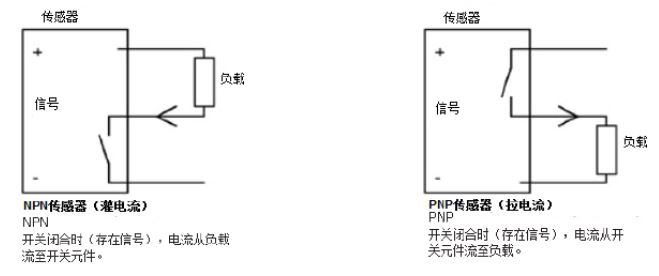
\includegraphics[width=0.6\textwidth]{fig_2_05i.jpg}
  \caption{NPN与PNP传感器}\label{fig_2_05i}
\end{figure}

\section{模拟量输入通道}

\subsection{模拟量输入通道的结构}

对于高速系统.特别是需要同时得到描述系统性能各项数据的系统,可采用图\ref{fig_2_06}所示并行转换结构。其特点是速度快、工作可靠,即使某一通路有故障,也不会影响其他通路正常工作。


\begin{figure}[h]
  \centering
  % Requires \usepackage{graphicx}
  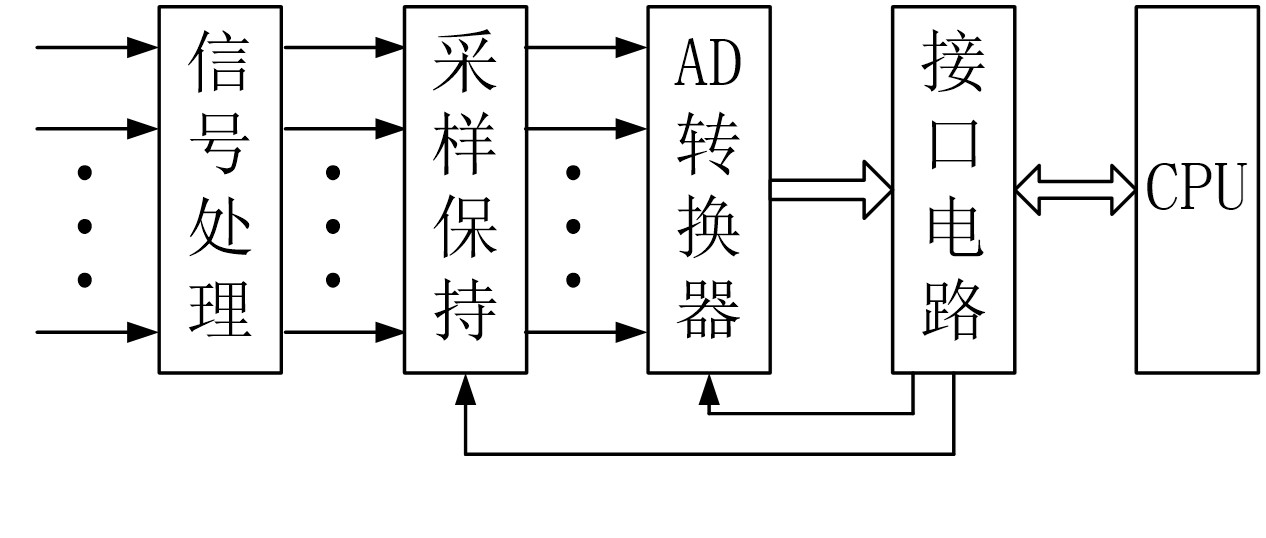
\includegraphics[width=0.4\textwidth]{fig_2_06}\\(a) 并行转换结构\\
  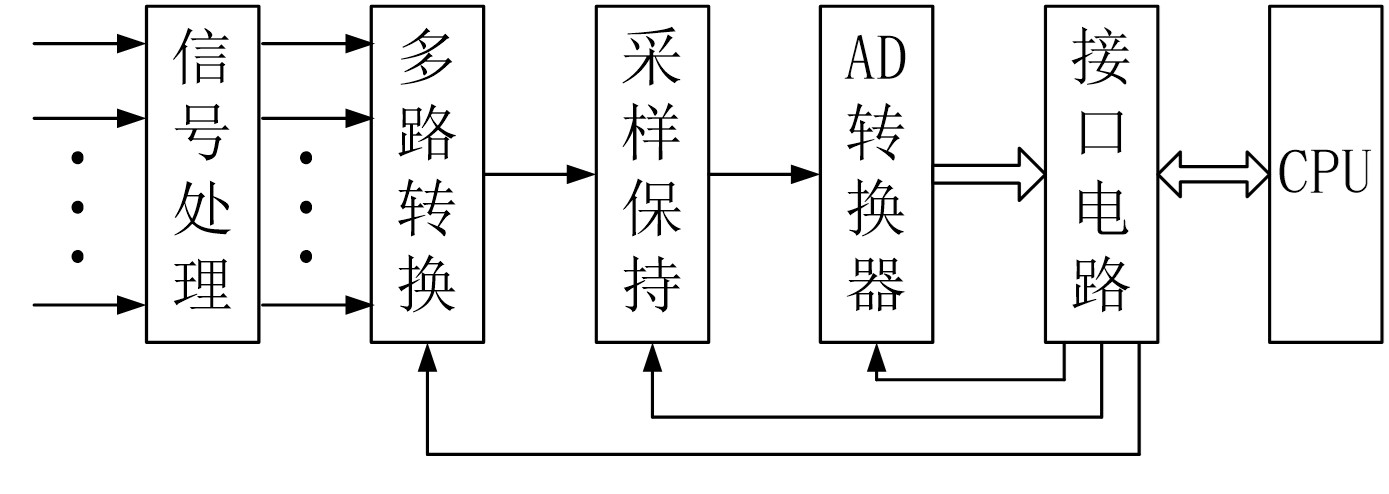
\includegraphics[width=0.4\textwidth]{fig_2_06a}\\(b) 串行(多路通道共享采样保持或模数转换电路)\\
  \caption{模拟量输入通道的结构}\label{fig_2_06}
\end{figure}




\subsection{信号处理}


\begin{itemize}
  \item 信号处理形式
  \begin{itemize}
    \item 信号大小

    \item 电压电流
  \end{itemize}

\begin{figure}[h]
  \centering
  % Requires \usepackage{graphicx}
  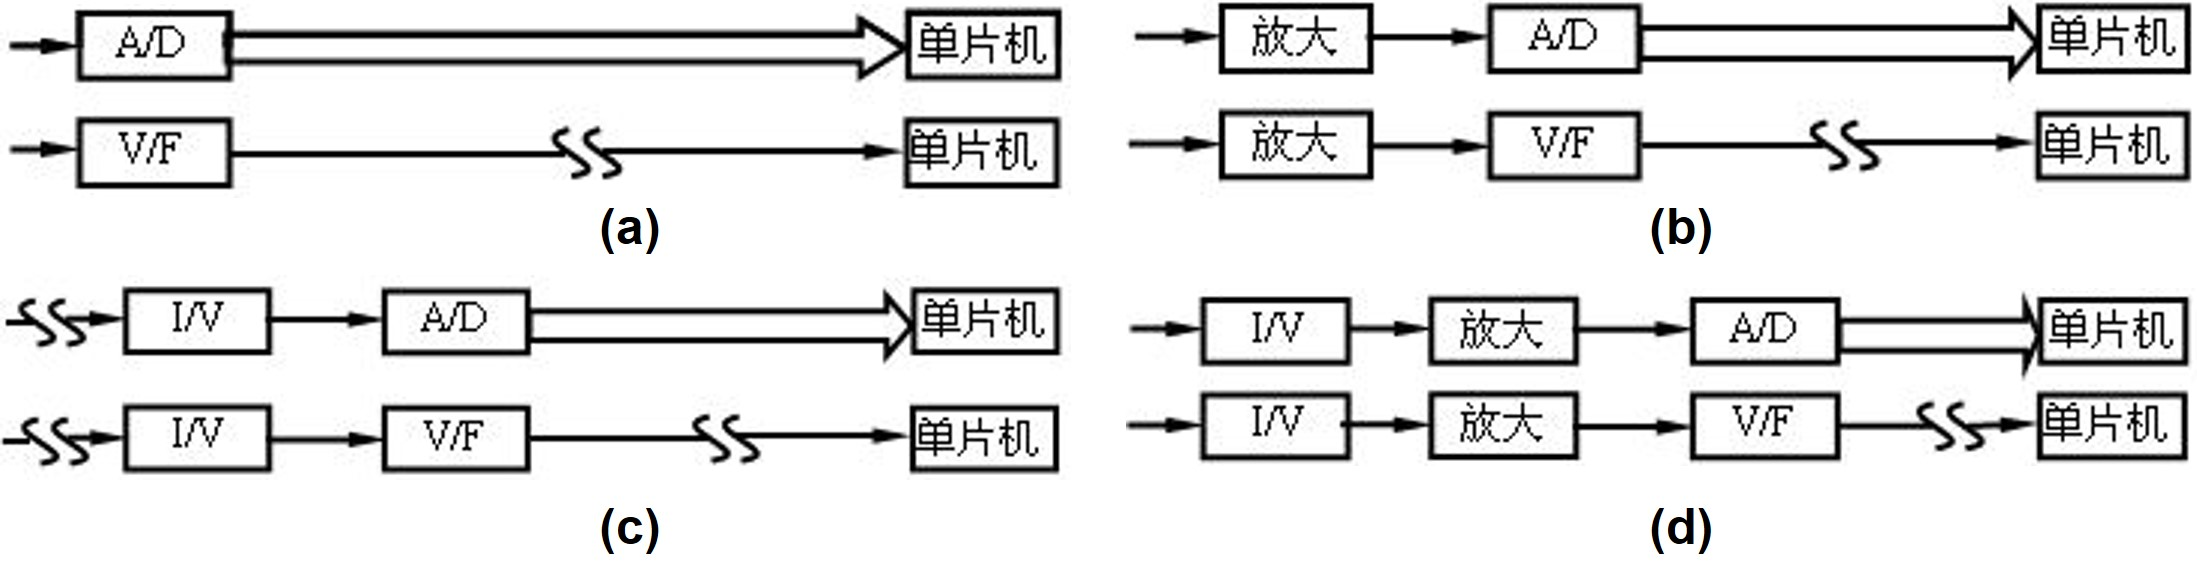
\includegraphics[width=0.8\textwidth]{fig_2_06b}
  \caption{针对不同信号的处理形式,(a)大电压,(b)小电压,(c)大电流,(d)小电流。}\label{fig_2_06b}
\end{figure}


  \item 常用放大电路
  \begin{itemize}
    \item 运算放大器的基本电路
    \item 仪表放大器
    \item 程控放大器
    \item 隔离放大器
  \end{itemize}
  \item I/V变换
  \begin{itemize}
    \item 无源
    \item 有源
  \end{itemize}
\end{itemize}


\subsection{采样保持}

AD转换器将模拟信号转换为数字量需要一定的时间,对于随时间变化的模拟信号来说,转换时间决定了每个采样时刻的最大转换误差。AD 转换延迟所引起的可能误差是$\Delta U$。 对于一定的转换时间,最大可能的误差发生在信号过零的时刻,因为此时dU/dt 最大,转换时间一定,所以$\Delta U$最大,如图\ref{fig_2_07}所示。


\begin{figure}[h]
  \centering
  % Requires \usepackage{graphicx}
  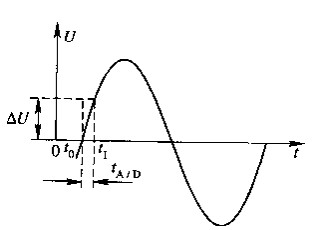
\includegraphics[height=0.15\textheight]{fig_2_07}
  \caption{正弦信号的采样保持}\label{fig_2_07}
\end{figure}


令$U=U_m sin \omega t$,则

\begin{equation}
  dU/dt  =U_m \omega cos \omega t =U_m 2\pi f cos 2\pi ft
\end{equation}

式中,$U_m$为正弦信号的幅值,$f$为信号频率,在坐标原点有:

\begin{equation}
  \Delta U/\Delta t = U_m  2\pi f
\end{equation}

取$\Delta t=t_{A/D}$,则得原点处转换的不确定电压误差为

\begin{equation}
  \Delta U = U_m  2\pi ft_{A/D}
\end{equation}

误差的百分数为:

\begin{equation}
  \sigma =  \Delta U/U_m \times 100\% = 2\pi ft_{A/D}\times 100\%
\end{equation}



实例:一个10位的AD转换器,若要求转换精度为$0.1\%$,转换时间为10μs,则允许转换的正弦波模拟信号的最大频率为

\begin{equation}
  f=\frac{0.1}{2\pi\times10\times10^{-6}\times10^2} \approx 16Hz
\end{equation}

采样/保持器一般由模拟开关、储能元件(电容)、输入和输出缓冲放大器组成。
    采样保持电路有两个工作状态, 一是采样状态.二是保持状态。

选择采样/保持器时,应考虑如下因素:
\begin{enumerate}
  \item 采样保持器的孔径时间:保持命令发出后K完全断开所需时间;

  \item 采样保持器的捕捉时间:由保持到采样时输出U,从原保持值过渡到跟踪信号的时间;

  \item 保持电压变化率:$dU/dt = I_D/C$,其中,$I_D$ 的漏电流。
   \item 常用的采样保持芯片:LF398

\end{enumerate}

应当指出,在模拟量输入通道中,只有在信号变化频率较高而A/D转换速度又不高,以致转换误差影响转换精度时,或者要求同时进行多路采样的情况下,才需要设置采样保持电路,对于一些变化缓慢的生产过程(如石油、化工等)可以不设置保持电路。



\subsection{多路转换器}

多路转换器又称多路开关是用来切换模拟电压信号的关键元件。利用多路开关可将各个输入信号依次地或随机地连接到公用放大器或A/D转换器上 。


\begin{figure}[h]
  \centering
  % Requires \usepackage{graphicx}
  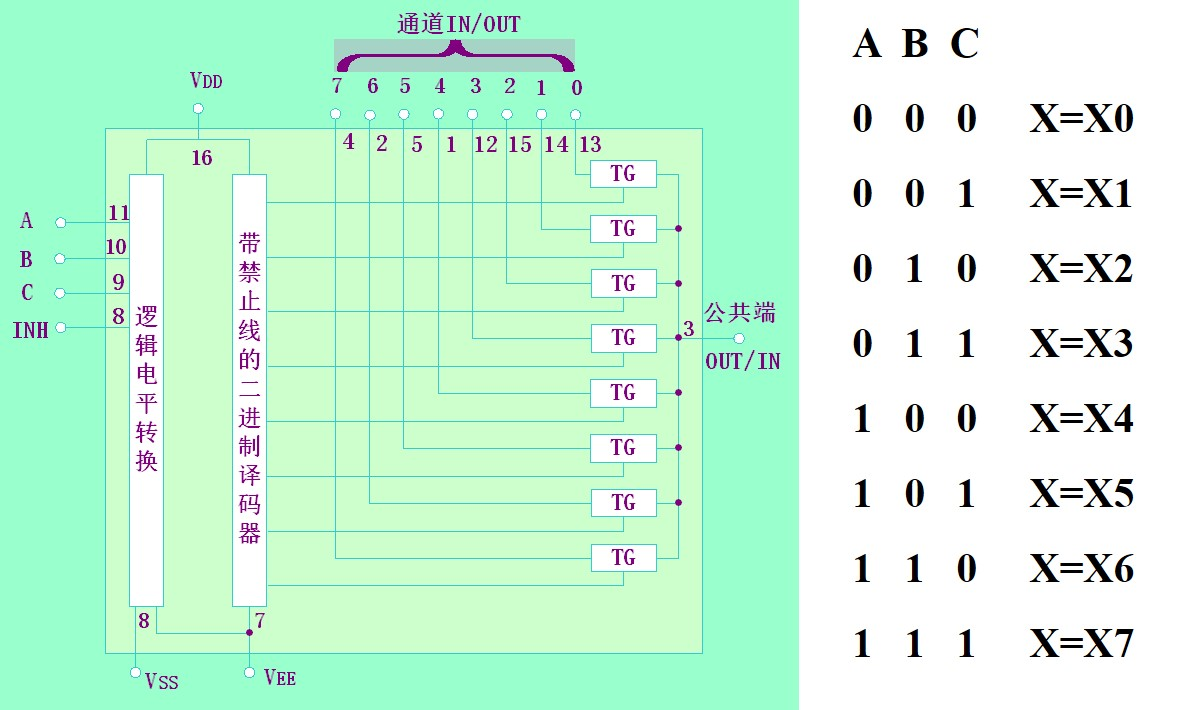
\includegraphics[width=0.6\textwidth]{fig_2_07a}\\
  \caption{多路开关CD4051}\label{fig_2_07a}
\end{figure}


\subsection{A/D转换技术}


\subsubsection{A/D转换原理(1)逐次逼近}

逐次逼近型A/D转换芯片中包括逐次逼近寄存器SAR、D/A转换器、比较器、时序及控制逻辑等部分组成如图\ref{fig_2_08}所示。


\begin{figure}[h]
  \centering
  % Requires \usepackage{graphicx}
  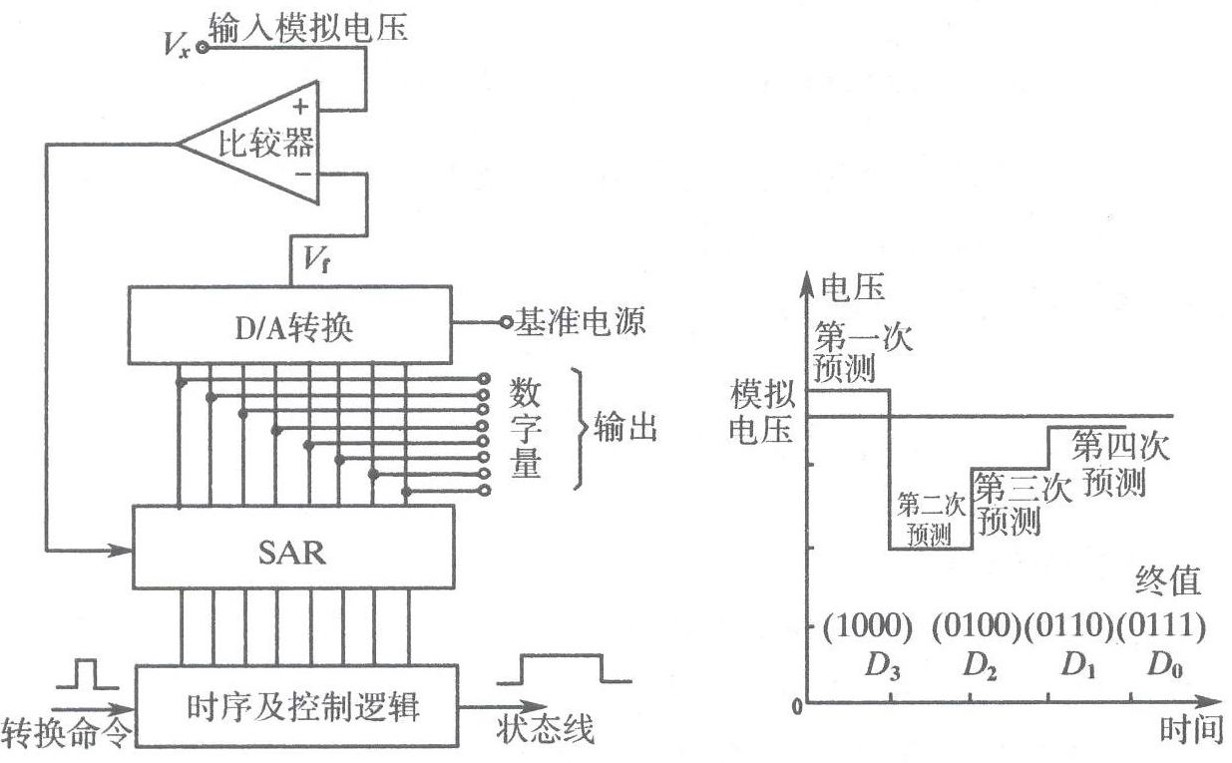
\includegraphics[width=0.6\textwidth]{fig_2_08}\\
  \caption{逐次逼近型A/D}\label{fig_2_08}
\end{figure}

转换过程如下:

\begin{enumerate}
  \item 时序及控制逻辑给SAR最高位为“1”,其余为“0”,经D/A转换为模拟电压Vf ,然后与输入电压Vx 比较,确定该位;
  \item 当Vx ≥Vf ,此位为“1”,置下位为“1”;
  \item 当Vx $<$ Vf ,此位为“0”,置下位为“1”。
  \item 按上述方法依次类推,逐位比较判断,直至确定SAR的最低位为止。
\end{enumerate}




\subsubsection{A/D转换原理(2)双斜率积分}

双斜率积分A/D:器件少、使用方便、抗干扰能力强、数据稳定、价格便宜。典型芯片:MC14433、AD7550、ICL7109\newline

如何理解双斜率积分A/D的工作原理?


首先,明确积分器输出与模拟输入电压之间的关系,如图\ref{fig_2_09} 所示。


\begin{figure}[h]
  \centering
  % Requires \usepackage{graphicx}
  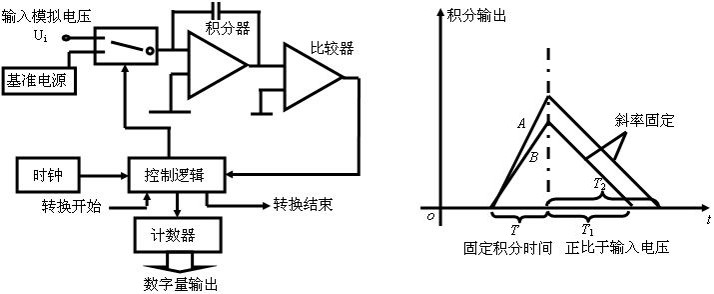
\includegraphics[width=0.6\textwidth]{fig_2_09}\\
  \caption{双斜率积分A/D}\label{fig_2_09}
\end{figure}

  其次,将A/D转换的过程分为两个阶段,即:
  \begin{enumerate}
    \item 模拟开关连接至模拟输入电压。由于模拟输入电压越大,积分器输出电压的变化率就越大。经过固定时间T后,不同大小的输入模拟电压UA、UB 就会达到不同的积分输出。

    \begin{equation}
    -\int_0^T\frac{U_i}{RC}dt=U_o-0
  \end{equation}

  得到


\begin{equation}\label{eq_2_1}
  U_o=-\frac{U_i}{RC}T
  \end{equation}

    \item 模拟开关切换至基准电源(与模拟输入电压极性相反)。由于基础电源的电压值固定,且与原输入电压极性相反,会使积分输出电压以固定斜率(由基准电源电压确定)下降,直至下降到0。 此过程中,利用计数器对这一时间段计时。
              \begin{equation}
    -\int_T^{T+T_1}\frac{U_{REF}}{RC}dt=0-U_o
  \end{equation}
      得到

   \begin{equation}\label{eq_2_2}
  U_o=\frac{U_i}{RC}T_1
  \end{equation}

      由式\ref{eq_2_1}和\ref{eq_2_2}得到:

  \begin{equation}
   -\frac{U_i}{RC}T=\frac{U_i}{RC}T_1
  \end{equation}

  推出:
    \begin{equation}
   {U_i}=-\frac{T_1}{T}U_{REF}
  \end{equation}

  即$U_i\propto T_1$



  \end{enumerate}

  易知:模拟输入电压与积分输出电压下降至0的时间为正比关系。因而,可用计数器的数字量输出表示输入电压的大小。







\subsubsection{A/D转换原理(3)$\Sigma-\Delta$型}

工作原理:模拟信号与1位DAC的输出送到减法器,经积分器后送到比较器。以Kfs采样速率将输入信号转换为由1和0构成的连续串行位流。精度最高的A/D转换器,一般说来速度较低。典型芯片:AD7715

\begin{figure}[h]
  \centering
  % Requires \usepackage{graphicx}
  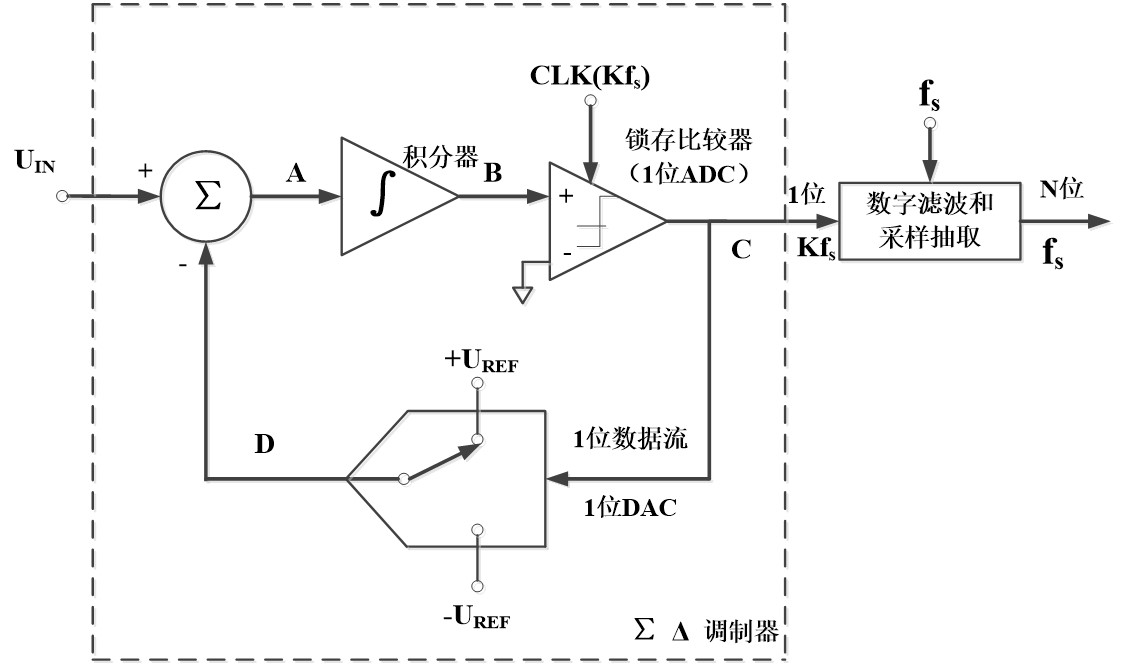
\includegraphics[width=0.6\textwidth]{fig_2_10}\\
  \caption{$\Sigma-\Delta$型A/D}\label{fig_2_10}
\end{figure}


\begin{figure}[h]
  \centering
  % Requires \usepackage{graphicx}
  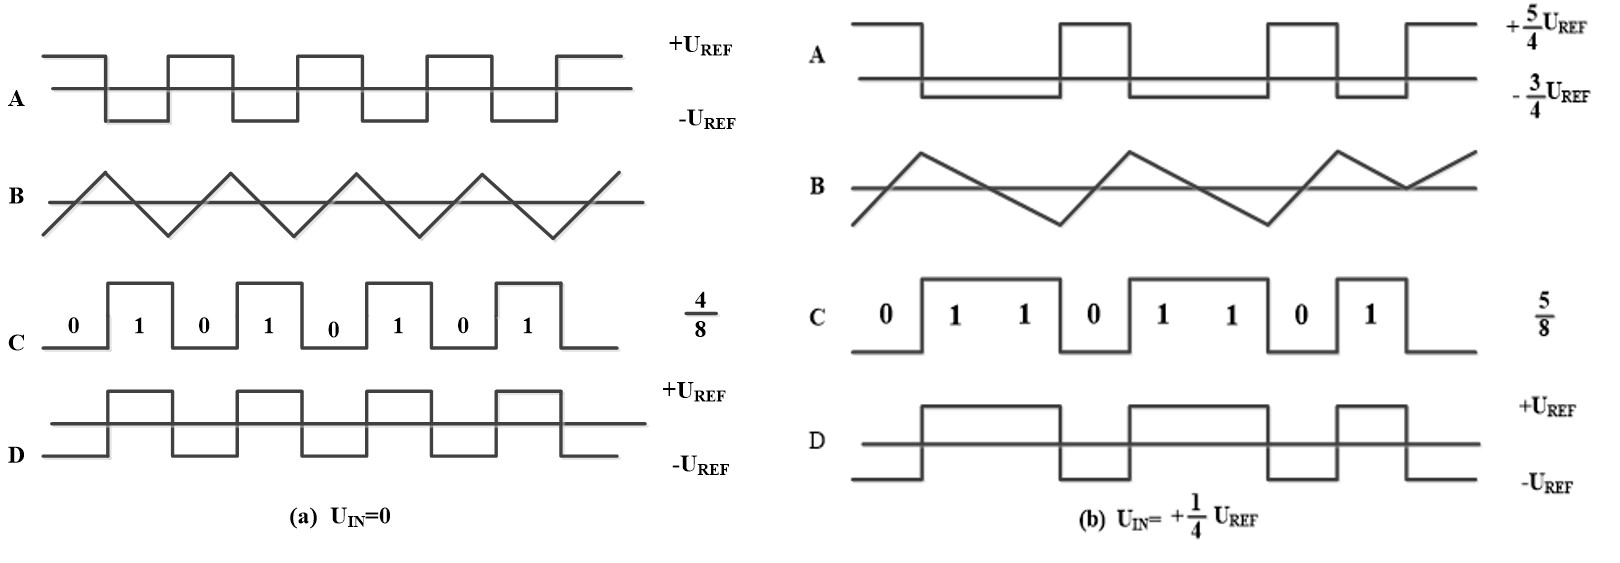
\includegraphics[width=0.9\textwidth]{fig_2_10a}\\
  \caption{$\Sigma-\Delta$型A/D举例}\label{fig_2_10a}
\end{figure}

\begin{remark}ADI公司提供的演示视频:

  http://designtools.analog.com/dt/sdtutorial/sdtutorial.html
\end{remark}


\subsubsection{A/D技术指标}



\begin{itemize}
  \item 分 辨 率

  分辨率通常用数字输出最低有效位(Least Significant Bit,LSB)所对应的模拟量输入电压值表示,例如:AD 位数n=8,满量程为5V,则LSB对应$5V/(2^8-1)=19.6mV$。
     由于分辨率直接与转换位数有关,所以一般也用其位数表示分辨率,如8,10、12、14、16为AD。
     通常把小于8位的称为低分辨率,10-12位的成为中分辨率,14位以上的为高分辨率。

  \item 转换时间

  从发出转换命令信号到转换结束信号有效的时间间隔,即完成一次转换所用的时间,为转换时间。转换时间的倒数为转换速率。
      通常转换时间从几ms到100ms成为低速,从几μs到100μs称为中速,从10ns到100ns左右成为高速。

  \item 转换量程

         所能转换的模拟量输入电压范围,如0-5V,-5 -+5V 等。

\end{itemize}



\subsubsection{A/D实现技术}

A/D转换器与CPU连接时需要考虑的问题

\begin{itemize}
  \item 输入模拟电压的连接
  \begin{itemize}
    \item 单端输入:IN直接与信号连接
    \item 差动输入:VIN(+) VIN(-)
    \begin{itemize}
      \item 单端输入正信号:UIN(+)接信号、UIN(-)接地
      \item 单端输入负信号: UIN(-)接信号、UIN(+)接地。

    \end{itemize}



  \end{itemize}




  \item 数据输出线和系统总线的连接
  \begin{itemize}
    \item 数据线具有可控三态输出门,可直接与系统总线连接;

    \item 数据线没有三态输出门或具有内部三态门但不受外部控制,则(不能直接连接系统总线)必须通过I/O接口连接;

    \item 8位以上A/D转换需考虑A/D的数据输出线和系统总线位数的对应关系(针对8位CPU、 12位A/D,需分高低位分别连接,分时按字节读入)。

        \begin{itemize}
    \item A/D位数=数据总线位数
    \item 	A/D位数$>$数据总线位数

    \item A/D位数$<$数据总线位数

  \end{itemize}
\end{itemize}




\end{itemize}






\section{模拟量输出通道}


\subsection{模拟量输出通道的结构}


一个实际的计算机控制系统中,往往需要多路的模拟量输出,其实现方法有两种:

\begin{enumerate}
  \item 数字保持式结构:一个通路一个D/A转换器,CPU 与D/A 之间通过独立的接口缓冲器传送信息。

      特点:速度快,精度高,可靠,互不影响;D/A多。

  \item 模拟保持式结构:多个通路共用一个D/A,CPU分时将各路D/A转换通过多路开关分送各路保持电路去。

特点:省D/A,速度慢,可靠性较差。

\end{enumerate}

\begin{figure}[h]
  \centering
  % Requires \usepackage{graphicx}
  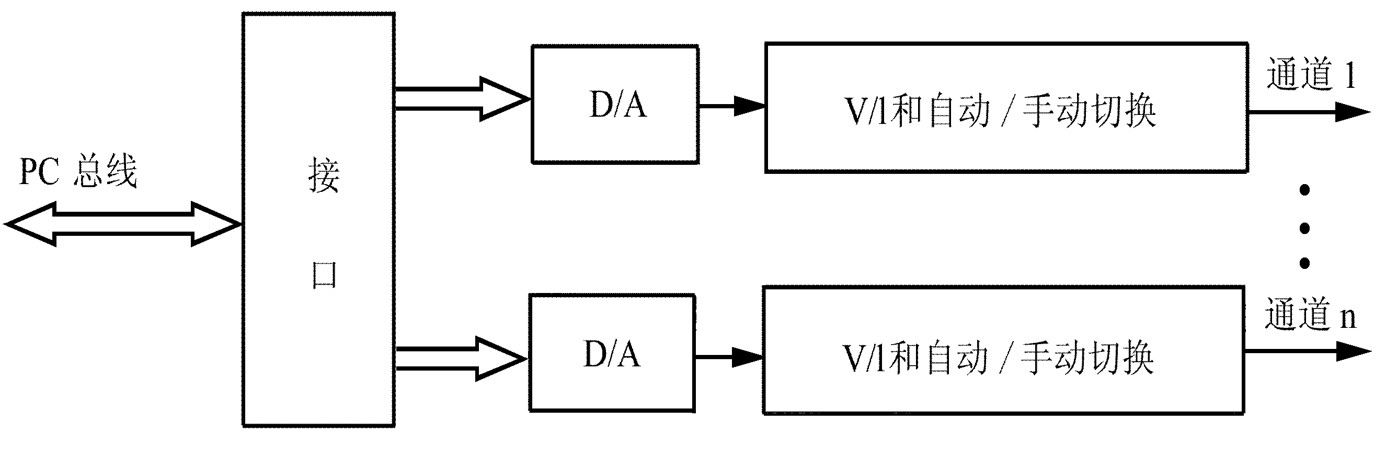
\includegraphics[width=0.6\textwidth]{fig_2_11}\\(a) 数字保持式\\
  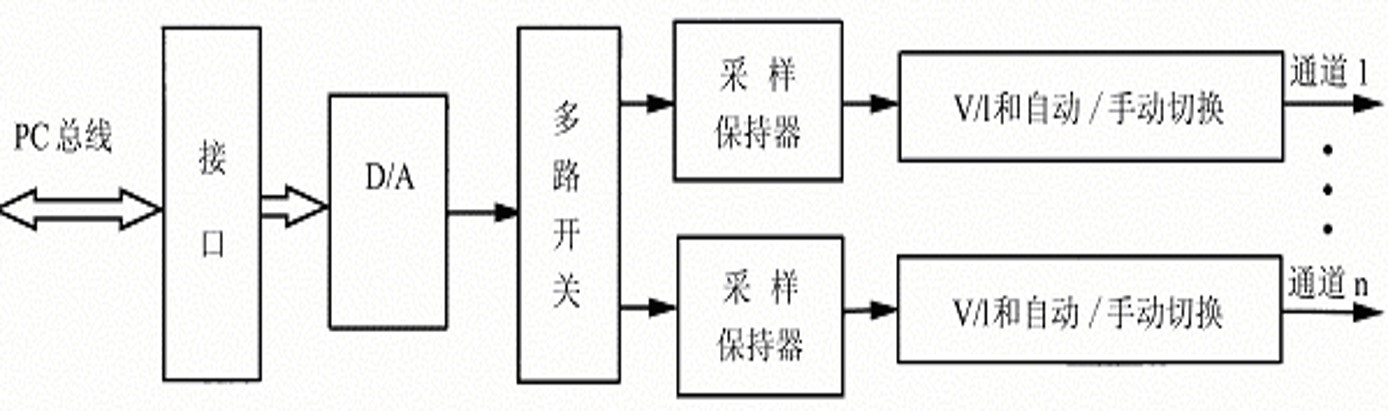
\includegraphics[width=0.6\textwidth]{fig_2_11a}\\(b) 模拟保持式
  \caption{模拟量输出通道的结构}\label{fig_2_11}
\end{figure}

\subsection{D/A转换技术}






\subsubsection{D/A转换原理(1)分类}

依据D/A转换原理不同可分为:

\begin{itemize}
\item 求取脉冲平均值的PWM型

\item 数字编码信号控制下加权量叠加型
\end{itemize}

加权量叠加型一般由四部分组成,即电子开关、电阻网络、放大器和标准电压源;根据电阻网络不同,可分为权电阻译码D/A转换器、倒T 型网络D/A转换器等,如图\ref{fig_2_12}、\ref{fig_2_12a}所示。



\subsubsection{D/A转换原理(2)权电阻D/A转换器}





图\ref{fig_2_12}所示权电阻D/A转换器,运算放大器的输入电流为:





\begin{equation}
  I = \sum_{i=0}^{n-1}I_i = \sum_{i=0}^{n-1} \frac{U_R}{2^{n-1}R}D_i2^i = \frac{U_R}{2^{n-1}R}\sum_{i=0}^{n-1} D_i2^i
\end{equation}


运算放大器的输出电压为:


\begin{equation}
  U=-IR_f  =-\frac{U_RR_f}{2^{n-1}R}\sum_{i=0}^{n-1} D_i2^i
\end{equation}

若$R_f = 1/2R$,代入上式得

\begin{equation}
  U=- \frac{U_RR_f}{2^{n-1}R}\sum_{i=0}^{n-1} D_i2^i = -\frac{U_R}{2^{n-1}}\sum_{i=0}^{n-1} D_i2^i
\end{equation}


当D/A的输入数据为0时,

\begin{equation}
  U=0
\end{equation}

当D/A的输入数据为$0x1...11H$时,

\begin{equation}
  U_m=-\frac{2^n-1}{2^n}U_R
\end{equation}

因而U的变化范围是

\begin{equation}
  0-\frac{2^n-1}{2^n}U_R
\end{equation}

\begin{figure}
  \centering
  % Requires \usepackage{graphicx}
  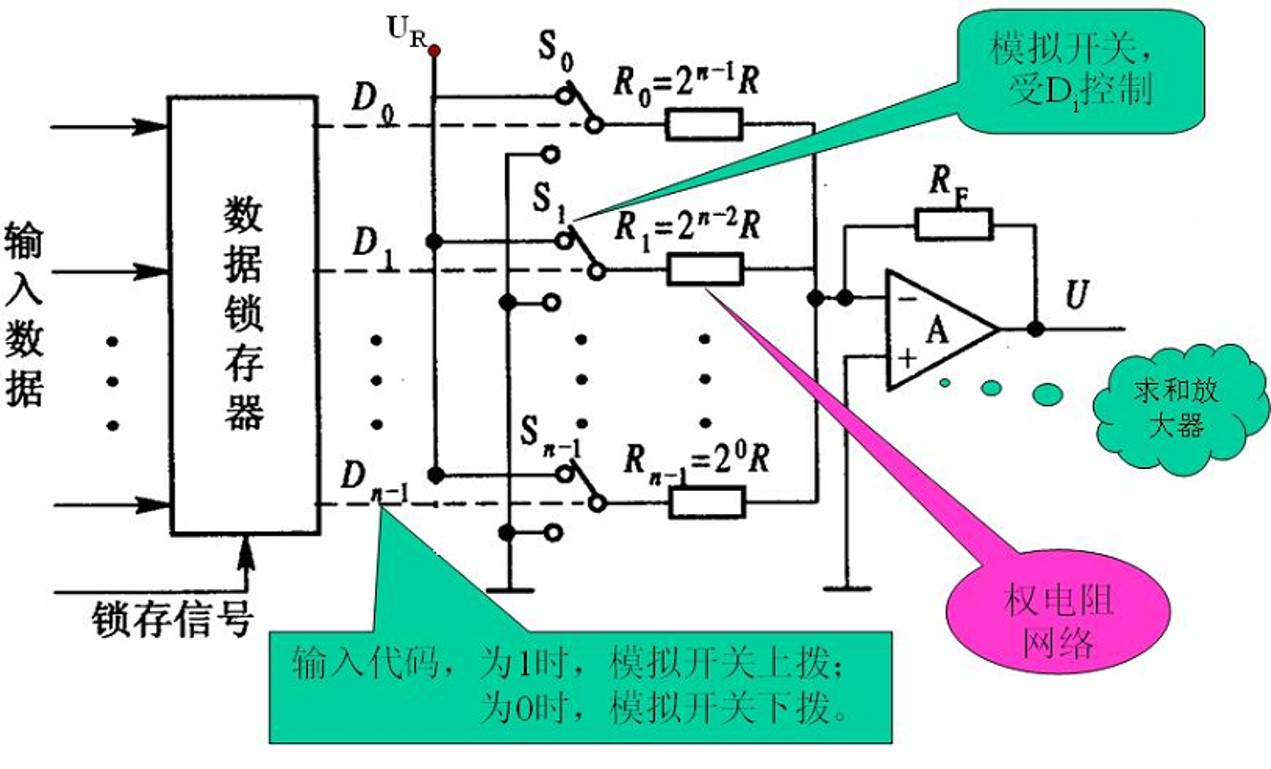
\includegraphics[width=0.5\textwidth]{fig_2_12}
  \caption{权电阻D/A}\label{fig_2_12}
\end{figure}


\subsubsection{D/A转换原理(3)倒T型网络D/A转换器}

如图\ref{fig_2_12a} 所示,Di=1,Si将电阻接到运放反向输入端;Di=0, Si将i将电阻接到运放同向输入端;都是虚地,各支路电流不会变化;流入2R支路的电流是以2的倍速递减;

\begin{eqnarray}
  I_\Sigma &=& D_{n-1}\frac{I}{2^1} +D_{n-2}\frac{I}{2^2}+...+D_{1}\frac{I}{2^{n-1}}+D_{0}\frac{I}{2^{n}}\\
&=&\frac{I}{2^{n}} (D_{n-1}2^{n-1} + D_{n-2}2^{n-2} + ... + D_{1}2^{1} + D_{0}2^{0})\\
&=&\frac{I}{2^{n}}\sum_{i=0}^{n-1} D_i2^i
\end{eqnarray}


运算放大器的输出电压为:

\begin{equation}
  U=-I_\Sigma R_f  =- \frac{IR_f}{2^{n}}\sum_{i=0}^{n-1} D_i2^i
\end{equation}

若$R_f=R$,并将$I=U_R/R$代入上式,则有
\begin{equation}
  U=-I_\Sigma R_f  =- \frac{U_R}{2^{n}}\sum_{i=0}^{n-1} D_i2^i
\end{equation}

可知,输出模拟电压正比于数字量的输入。



\begin{figure}
  \centering
  % Requires \usepackage{graphicx}
  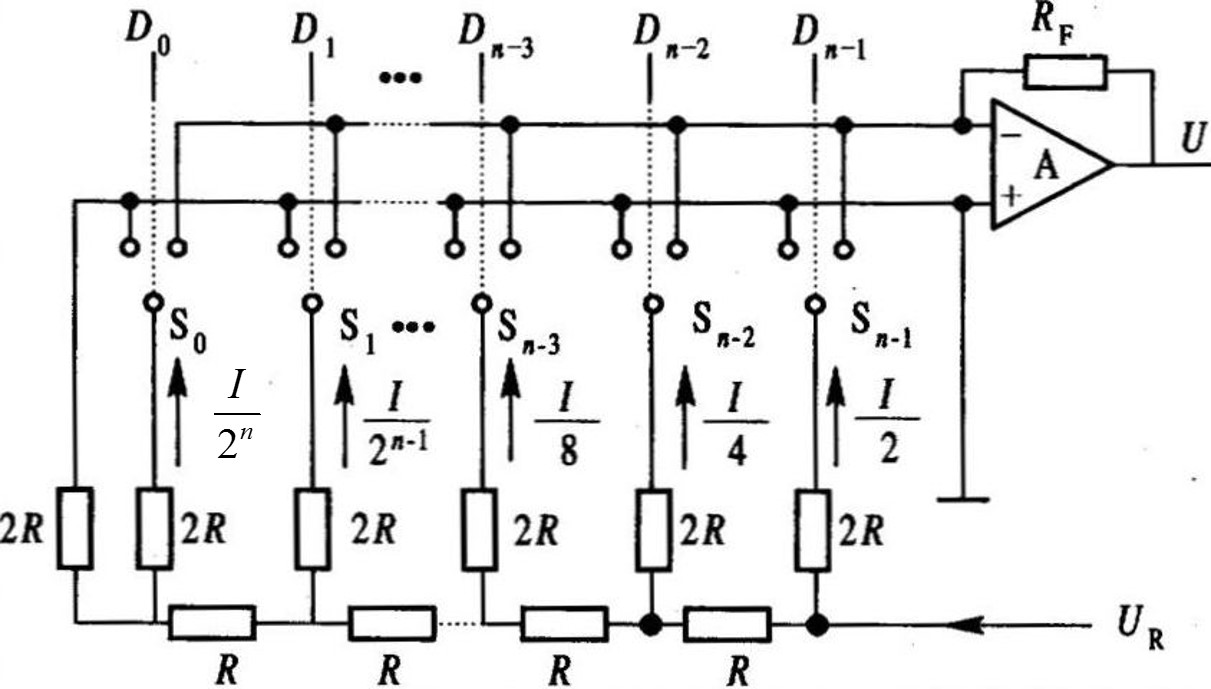
\includegraphics[width=0.5\textwidth]{fig_2_12a}
  \caption{倒T型网络D/A转换器}\label{fig_2_12a}
\end{figure}


\subsubsection{D/A技术指标}


\begin{description}
  \item[分 辨 率] 与A/D转换器的分辨率概念类似,指当输入数字量变化1时,输出模拟量变化的大小。分辨率通常用数字量的位数来表示,如8 位、12位、18 位。
  \item[稳定时间] 指D/A转换器所有输入二进制数变化是满刻度时,模拟量输出稳定到±1/2LSB范围内所需要的时间。一般为几十纳秒到几微秒完程一次转换所需要的时间;

  \item[线 性 度] 一个理想的D/A转换器输入输出特性应是线性的。在满量程范围内,偏离理想转换特性的最大误差称为线性误差,一般用LSB的分数表示。
\end{description}




\subsubsection{D/A实现技术}


如图\ref{fig_2_13}所示为DAC0832的原理图。
在使用DAC0832时应注意以下两个内容:

\begin{figure}
  \centering
  % Requires \usepackage{graphicx}
  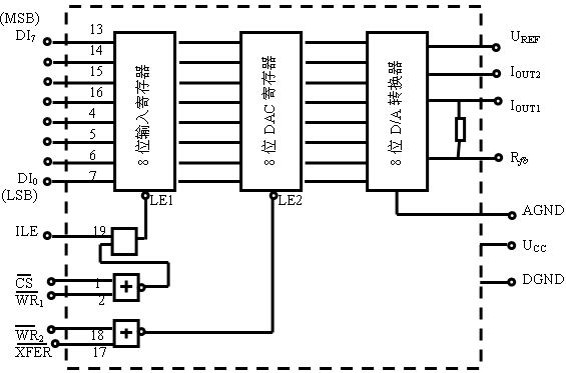
\includegraphics[width=0.5\textwidth]{fig_2_13}
  \caption{DAC0832}\label{fig_2_13}
\end{figure}


\begin{itemize}
  \item 极性:如图\ref{fig_2_14}所示;
  \item 与CPU接口--缓冲方式:如图\ref{fig_2_15}所示。
\end{itemize}

\begin{figure}
  \centering
  % Requires \usepackage{graphicx}
  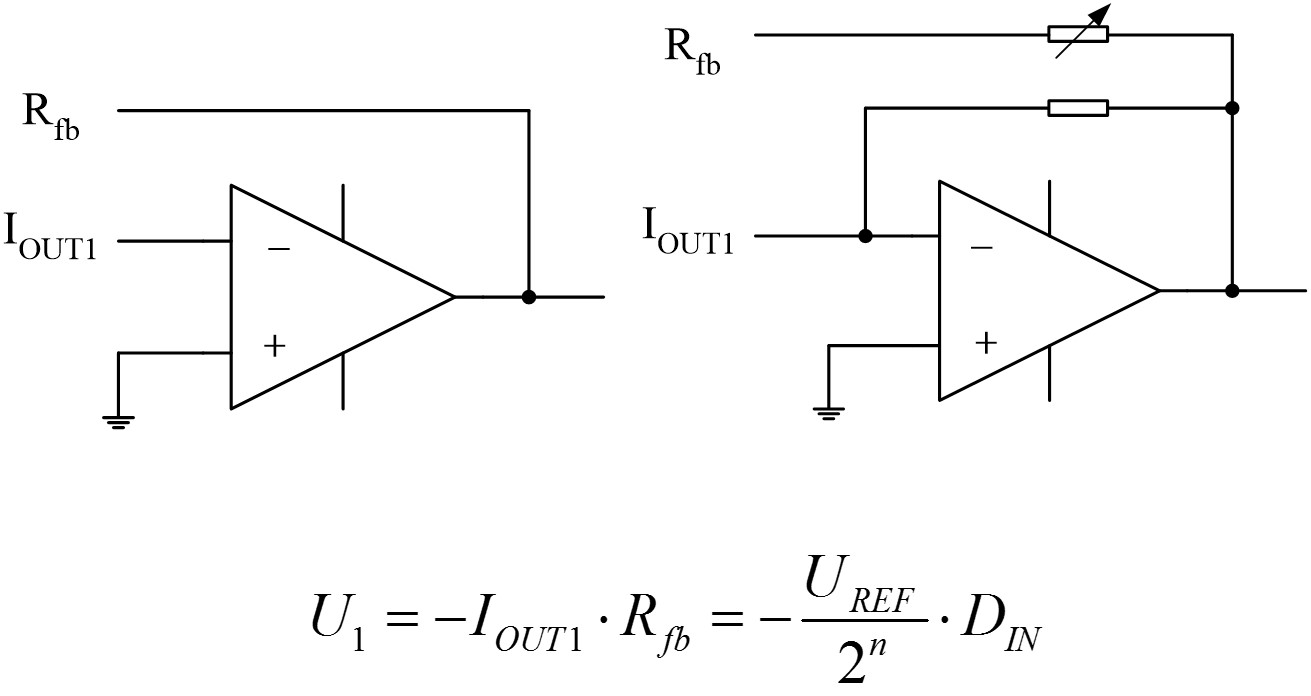
\includegraphics[width=0.45\textwidth]{fig_2_14}(a)
  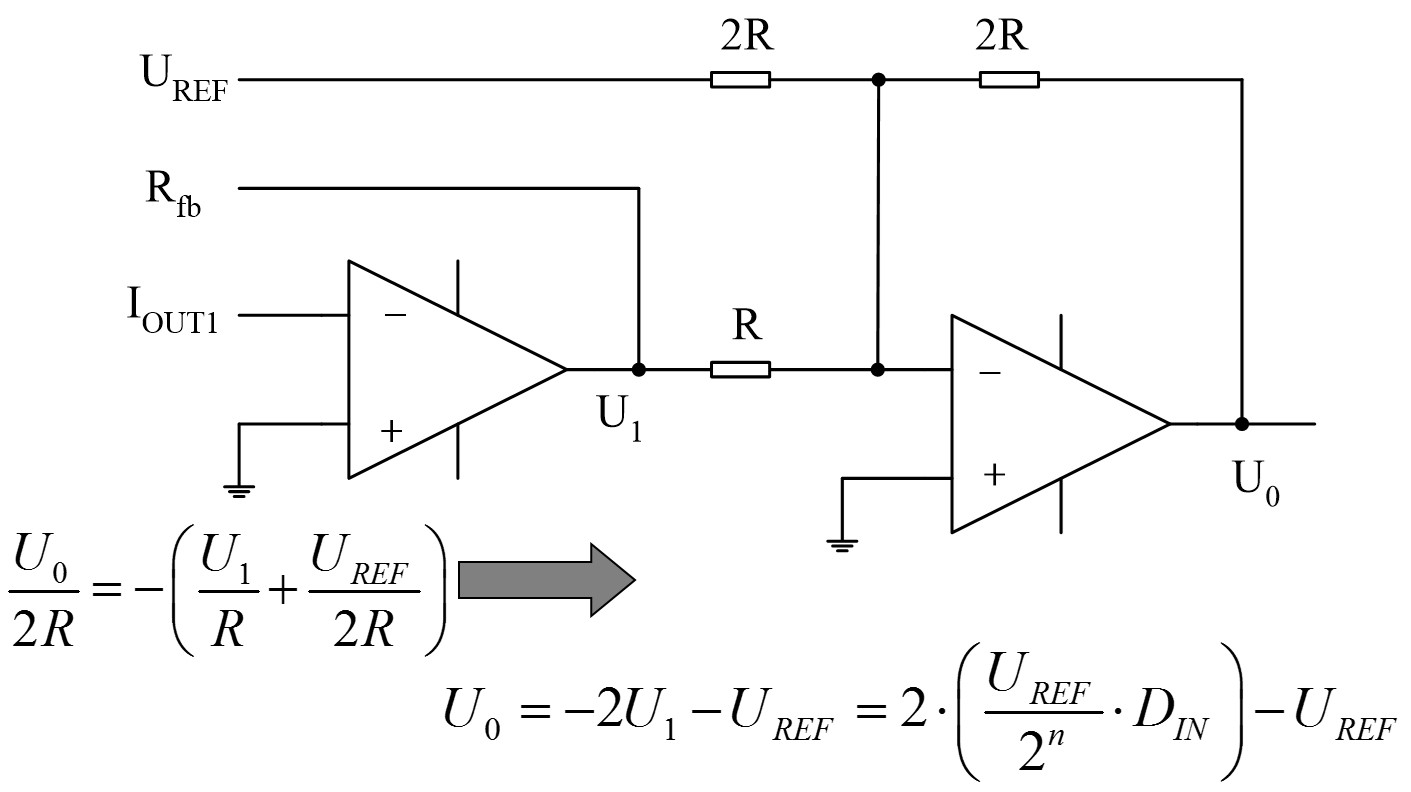
\includegraphics[width=0.45\textwidth]{fig_2_14a}(b)
  \caption{模拟输出极性变换}\label{fig_2_14}
\end{figure}


\begin{figure}
  \centering
  % Requires \usepackage{graphicx}
  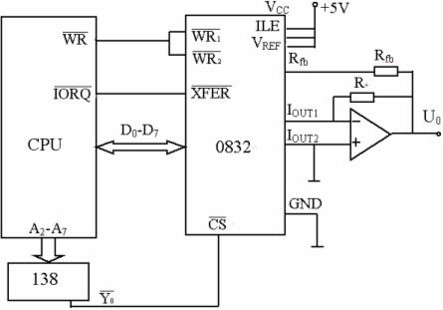
\includegraphics[width=0.45\textwidth]{fig_2_15}(a)
  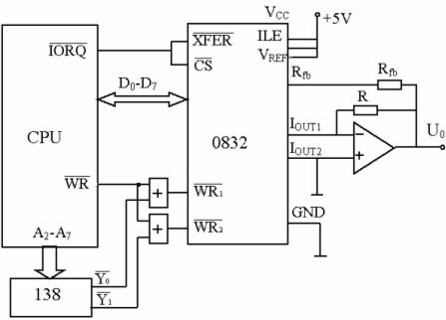
\includegraphics[width=0.45\textwidth]{fig_2_15a}(b)
  \caption{与CPU的接口---缓冲方式}\label{fig_2_15}
\end{figure}






\section{本章要点总结}

\begin{itemize}

\item 过程通道的概念及组成;
\item 编址方式的种类和特点;
\item 常用的地址译码方法,重点理解译码器译码的设计方法;
\item 总线接口常用芯片的使用;
\item 数字量输入通道的结构,并了解其信号调理方式;
\item 数字量输出通道的结构,并了解其输出调理电路设计;
\item 模拟量输入通道的结构,常见到信号处理形式;
\item 了解信号放大,I/V变换的种类以及原理;
\item 理解采样保持的使用以及采样/保持器的概念和作用;
\item 逐次逼近式和双积分式A/D转换的原理;
\item A/D转换器的技术指标;
\item A/D转换器与计算机的接口方法;
\item 模拟量输出通道的一般结构和特点;
\item 权电阻和倒T型网络D/A转换器原理;
\item D/A转换器的技术指标;
\item DAC0832与CPU的接口方法及输出极性的变换;


\end{itemize}
